\section{Multilinearity}
\label{sec:multi}

In this section we develop an extension of the transposition theorem
to the multilinear case.  The subject has already been treated by
Hopcroft and Musinski \cite{hopcroft+musinski73} and Fiduccia
\cite{fiduccia:phd}, this section is a mild generalization of their
methods.

\subsection{Multilinear circuits}
\label{sec:multilinear-circuits}
We shall consider \index{multilinear~circuit}\emph{multilinear
  circuits}, i.e. circuits that, besides the operators
of~\eqref{eq:tbasis}, also contain binary multiplication nodes. The
definitions of the previous section must be adapted to deal with
operators that are not module morphisms, but this generalization is
straightforward (see also Appendix~\ref{cha:basic-categ-theory} for a
clean way of defining arithmetic circuits that supports both linear
and arbitrary circuits).

Multilinear circuits are constructed using the
\index{standard~multilinear~basis}\emph{standard multilinear basis}
$\Sbasis$
\begin{equation}
  \label{eq:sbasis}
  \tag{$\Sbasis$}
  \begin{aligned}
    + : R\times R &\ra R\text{,}    & * : R\times R &\ra R\text{,} &  \hub : R &\ra R\times R\text{,}\\
        a, b &\mapsto a+b\text{,}   &     a, b &\mapsto ab\text{,} &         a &\mapsto a,a\text{,}\\ \\
    \eta_a : \{\bom\} &\ra R\text{,}     &&& \omega : R &\ra \{\bom\}\text{,} \\
          \bom &\mapsto a\text{,} &&&          a &\mapsto \bom\text{.}
  \end{aligned}
\end{equation}


We are going to define a transformation process that transforms a
circuit over $(R,\Sbasis)$ in a (uniform) circuit family over
$(R,\Tbasis)$. We call this process \emph{linearization}, a special
case of it has been used in \cite{gashkov+gashkov05,sergeev08} to
transpose circuits that compute differentials.

\begin{definition}[Zero edge, null edge]
  Let $C$ be a circuit over $(R,\Sbasis)$, a \emph{zero edge} is any
  edge $e$ in $C$ such that one of the following conditions holds:
  \begin{itemize}
  \item $e$ stems from a node $v$ with $\beta(v)=\eta_0$, such an edge
    is also called a \emph{normal} zero edge;
  \item $e$ stems from a node $v$ with $\beta(v)=+$ and whose incident
    edges are both zero;
  \item $e$ stems from a node $v$ with $\beta(v)=*$ and such that at
    least one of the incident edges of $v$ is zero;
  \item $e$ stems from a node $v$ with $\beta(v)=\hub$ and whose input
    edge is zero.
  \end{itemize}
  A \emph{null edge} is any edge $e$ such that one of the following
  conditions holds:
  \begin{itemize}
  \item $e$ is incident to a node $v$ with $\beta(v)=\omega$, such an
    edge is also called a \emph{normal} null edge;
  \item $e$ is incident to a node $v$ with $\beta(v)=\hub$ and whose
    stemming edges are both null;
  \item $e$ is incident to a node $v$ with $\beta(v)\in\{+,*\}$ such
    that its stemming edge is null.
  \end{itemize}
  An output node whose incident edge is zero is called a \emph{zero
    output}, an input node whose stemming edge is null is called a
  \emph{null input}.  A \emph{normal} circuit is a circuit whose zero
  and null edges are all normal.
\end{definition}

Notice that the evaluation of a zero edge or output is the zero
function, the converse is not true.  There is an obvious normalization
technique that takes a generic circuit and transforms it in a normal
circuit having the same evaluation; clearly, the normalization does
not increase the size and the depth of the circuit (it generally
increases $\size_{\{\eta_0,\omega\}}$, though). When necessary, we
will restrict ourselves to normal circuits.

\begin{definition}[Linearization]
  \index{linearization}
  Let $C=(V,E)$ be a circuit over $(R, \Sbasis)$. Let $0=\{v\in
  V|\beta(v)=\eta_0\}$, a linearization of $C$ is a subset
  $\ell\subset\inp(C)\cup 0$ such that:
  \begin{itemize}
  \item for every $v\in V$ with $\beta(v)=+$ either none of its
    incident edges is reachable from $\ell$, or both are;
  \item for every $v\in V$ with $\beta(v)=*$ at most one of the edges
    incident to $v$ is reachable from $\ell$; if $R$ is
    non-commutative, such edge is always the left (right) edge and the
    linearization is called a \emph{left (right) linearization}.
  \end{itemize}
  The elements of $\ell\cap\inp(C)$ and $s = \inp(C) - \ell$ are
  respectively called the \index{linear~input}\emph{linear} and
  \index{scalar~input}\emph{scalar} inputs. An edge reachable from
  $\ell$ is called \index{linear!edge}\emph{linear},
  \index{scalar~edge}\emph{scalar} otherwise.
\end{definition}


\begin{definition}[Linearized circuit, scalar part]
  Let $C=(V,E,\le,\le_i,\le_o)$ be a normal circuit over $(R,\Sbasis)$
  and let $\ell$ be a linearization; without loss of generality, we
  suppose that all the scalar inputs precede the linear inputs in the
  ordering of $V$ (one can always permute inputs). Let $n$ be the
  number of scalars for the linearization $\ell$ and let
  $x_1,\ldots,x_n$ be distinct indeterminates over $R$. The
  \index{linearized~circuit}\emph{linearized circuit}
  $C_\ell=(V_\ell,E_\ell,\le_\ell,\le_{i,\ell},\le_{o,\ell})$ is the
  circuit over $(R[x_1,\ldots,x_n], \Tbasis)$
  (resp. $(R^\op[x_1,\ldots,x_n],\dual{\Tbasis})$) obtained from $C$
  as follows:
  \begin{itemize}
  \item $E_\ell$ is the subset of $E$ containing the linear edges,
  \item $V_\ell$ are the nodes of $V$ adjacent to $E_\ell$, where
    $\beta(v)$ has incurred the following substitutions:
    \begin{itemize}
    \item $\eta_0$ becomes $0$; $+, \hub, \omega$ are preserved;
    \item if $\beta(v)=*$, let $e$ be the only non-linear edge
      incident to $v$ and let
      $a=\eval_e(x_1,\ldots,x_n,\bullet,\ldots,\bullet)$, then $*$
      becomes $\rmul{a}$ (resp. $\lmul{a}$) if $e$ is the right
      (resp. left) incident edge to $v$;
    \item The ordering are the restriction to $V$ of the original
      ones.
    \end{itemize}
  \end{itemize}

  The sets $V-V_\ell$ and $E-E_\ell$ are called the \emph{scalar part}
  of $C$.
\end{definition}

Observe that non-linear edges do not depend on linear inputs, thus the
substitution for $*$ is well defined. Figure \ref{fig:linearization}
shows an example of linearized circuit (in the case $R$ is
commutative), we gray out the scalar part of the circuit.

\begin{figure}[!ht]
  \centering
  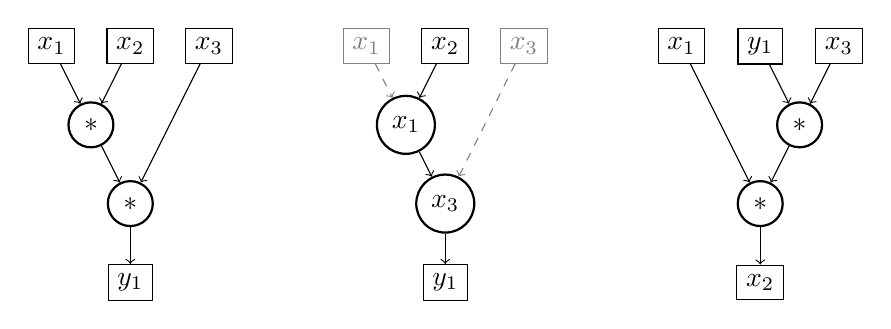
\begin{tikzpicture}
    \tikzstyle{node}=[circle,thick,draw=black,minimum size=4mm]
    \tikzstyle{arg}=[rectangle,thin,draw=black,minimum size=4mm]
    \tikzstyle{nodeg}=[circle,thick,draw=gray,minimum size=4mm]
    \tikzstyle{argg}=[rectangle,thin,draw=gray,minimum size=4mm]
    
    \begin{scope}
      \node[arg](in1){$x_1$};
      \node[arg,right of=in1](in2){$x_2$};
      \node[arg,right of=in2](in3){$x_3$};
      \node[node,below of=in1,xshift=5mm](times1){$*$};
      \node[node,below of=times1,xshift=5mm](times2){$*$};
      \node[arg,below of=times2](out){$y_1$};

      \path[->]
      (in1) edge (times1)
      (in2) edge (times1)
      (times1) edge (times2)
      (in3) edge (times2)
      (times2) edge (out);
    \end{scope}

    \begin{scope}[xshift=4cm]
      \node[argg](in1){\color{gray}{$x_1$}};
      \node[arg,right of=in1](in2){$x_2$};
      \node[argg,right of=in2](in3){\color{gray}{$x_3$}};
      \node[node,below of=in1,xshift=5mm](times1){$\rmul{x_1}$};
      \node[node,below of=times1,xshift=5mm](times2){$\rmul{x_3}$};
      \node[arg,below of=times2](out){$y_1$};

      \path[->]
      (in2) edge (times1)
      (times1) edge (times2)
      (times2) edge (out);
      
      \path[->,draw=gray,dashed]
      (in1) edge (times1)
      (in3) edge (times2);
    \end{scope}

    \begin{scope}[xshift=8cm]
      \node[arg](in1){$x_1$};
      \node[arg,right of=in1](in2){$\dual{y_1}$};
      \node[arg,right of=in2](in3){$x_3$};
      \node[node,below of=in3,xshift=-5mm](times1){$*$};
      \node[node,below of=times1,xshift=-5mm](times2){$*$};
      \node[arg,below of=times2](out){$\dual{x_2}$};

      \path[->]
      (in2) edge (times1)
      (times1) edge (times2)
      (times2) edge (out)
      (in1) edge (times2)
      (in3) edge (times1);
    \end{scope}
  \end{tikzpicture}
  \caption{A circuit over a commutative ring, its linearization for
    $\ell=\{x_2\}$ (scalar edges are grayed out) and its
    $\ell$-dual.}
  \label{fig:linearization}
\end{figure}

Any linearized circuit obviously defines an uniform circuit family
over $(R,\Tbasis)$ (resp. $(R^\op,\dual{\Tbasis})$), thus we can apply
the transposition theorem to the family. But there's more: from a
linearized circuit we can deduce a new circuit over $(R,\Sbasis)$ that
computes the same function as the transposed family.

\begin{definition}[$\ell$-dual]
  \label{def:ell-dual}\index{arithmetic~circuit!l-dual@$\ell$-dual}
  Let $C$ be a normalized circuit over $(R,\Sbasis)$ and let $\ell$ be
  a linearization.  The $\ell$-dual of $C$ is the circuit over
  $(R,\Sbasis)$ obtained by dualizing the linearized circuit $C_\ell$,
  then connecting back the edges of the scalar part to the
  corresponding nodes in $C_\ell$: in doing this nodes with
  $\beta(v)=\rmul{a}$ are changed back to $\beta(v)=*$; if the scalar
  edge was incident to the left (right) in $C$, it becomes incident to
  the right (left). The order on the nodes of the $\ell$-dual is
  arbitrary.
\end{definition}

By abuse of notation, the $\ell$-dual will also be noted
$\dual{C_\ell}$. Figure \ref{fig:linearization} shows an example of
$\ell$-dual; notice that $\dual{C_\ell}$ is only defined up to
reordering of the nodes, we will adopt the convention of preserving
the ordering of the linearized circuit, while we take the freedom to
permute the scalar part as it will be more convenient.

\begin{proposition}
  The size of the $\ell$-dual is the same as that of $C$, more
  precisely
  \begin{align*}
    \size_{\{+,\hub\}}(C) &= \size_{\{+,\hub\}}(\dual{C_\ell}), 
    &\size_{\{*\}}(C) &= \size_{\{*\}}(\dual{C_\ell}),\\
    \size_{\{\eta_0,\omega\}}(C) &= \size_{\{\eta_0,\omega\}}(\dual{C_\ell}), 
    &\size_{\{\eta_a|a\ne0\}}(C) &= \size_{\{\eta_a|a\ne0\}}(\dual{C_\ell}).
  \end{align*}
  Its depth is at most twice that of $C$.
\end{proposition}


\subsection{Bilinear chains}
\label{sec:bilinear-chains}

The case of bilinear circuits has received particular interest because
it permits to give lower bounds on the complexity of matrix
multiplication~\cite{fiduccia:phd}. In this section we just point out
how the results of Hopcroft and Musinski~\cite{hopcroft+musinski73}
and Fiduccia~\cite{fiduccia:phd} reduce to ours.

\begin{definition}[Linear chain]
  Let $R$ be non-commutative and let $S\subset R$ be a subring of its
  center. A circuit $C$ over $(R,\Tbasis)$ such that no directed path
  in $C$ contains two nodes $v\ne v'$ with $\beta(v)=\rmul{a}$ and
  $\beta(v')=\rmul{a'}$ where $a,a'\not\in S$ is called an
  \index{linear~chain}\emph{$S$-linear chain}.
\end{definition}

We have seen in Remark~\ref{rk:tellegen} that in the non commutative
case the transposition principle does not \emph{transpose
  matrices}. It is however possible to transpose linear chains.

\begin{definition}[Opposite circuit]
  Let $C=(V,E)$ be a circuit over $(R,\Tbasis)$, the
  \index{arithmetic~circuit!opposite}\emph{opposite circuit} of $C$,
  noted $C^\op$, is the arithmetic circuit over $(R^{\op},\Tbasis)$
  where any $\beta(v)=\rmul{a}$ has been changed to $\rmul{a^\op}$.
\end{definition}

\begin{proposition}
  Let $C$ be a linear chain and let $\eval_C(x)=\trans{x}M$ for some
  matrix $M$, then $\eval_{C^\op}(x)=\trans{M}x$.
\end{proposition}
\begin{proof}
  This is a consequence of the
  \hyperref[th:electrical-network]{electrical network lemma}.  The
  matrix $M$ associated to $\eval_C$ is given by
  \begin{equation}
    \label{eq:243}
    m_{ij} = \pi_j\circ\eval_C\circ\iota_i(1)
    = \sum_{p\in x_i\leadsto y_j}\eval_p(1) =
    \sum_{p\in x_i\leadsto y_j} p_1p_2\cdots p_{n_p}
    \text{,}
  \end{equation}
  where $\rmul{p_1},\ldots,\rmul{p_{n_p}}$ are the scalar
  multiplication nodes on the path $p$.

  Now, by the definition of linear chain, on any path there is at most
  one element not in the center of $R$, thus
  \begin{equation}
    \label{eq:245}
    p_1p_2\cdots p_{n_p}=p_{n_p}\cdots p_2p_1
    \text{,}
  \end{equation}
  and the claim follows.
\end{proof}

Thus, to any linear chain one can associate the four circuits
$C,\dual{C},C^\op,\dual{{C^\op}}$. In~\cite{hopcroft+musinski73,fiduccia:phd},
bilinear chains are considered, i.e.  bilinear circuits whose only two
linearizations are linear chains. The opposite circuit of a
\index{bilinear~chain}bilinear chain is defined by swapping every
multiplication node. Thus, if $C$ is a bilinear chain and
$\ell_1,\ell_2$ its linearizations, one obtains the six circuits
\[C,C^\op,\dual{C_{\ell_1}},\dual{{C_{\ell_1}^\op}},\dual{C_{\ell_2}},\dual{{C_{\ell_2}^\op}}\text{.}\]

Finally, the complexity bounds of~\cite{hopcroft+musinski73}, are
obtained by considering the sets $D=\{\rmul{a}|a\in S\}$ and
$M=\{\rmul{a}|a\not\in S\}$ and realizing that both $\size_D$ and
$\size_M$ are preserved taking the $\ell$-dual and/or the opposite.



% Local Variables:
% mode:flyspell
% ispell-local-dictionary:"american"
% mode:TeX-PDF
% mode:reftex
% TeX-master: "../these"
% End:
%
